\chapter{Rekayasa Genetika dan Bioteknologi}\label{ch:b3:genetic-engineering}

Sampai tahun 1982 setiap penyandang diabetes di dunia dipertahankan hidup oleh
insulin yang diekstraksi dari pankreas babi dan sapi --- sekitar delapan ribu
kilogram kelenjar bagi satu kilogram hormon --- dan sebagian pasiennya bereaksi
terhadap protein asing itu. Pada tahun itu obat pertama yang dibuat organisme
hasil rekayasa genetika sampai ke pasar: insulin manusia, yang disintesis
\emph{Escherichia coli} yang membawa gen manusia itu pada sebuah \omterm{def:b3:genetic-engineering:tools}{plasmid}.
Perkakas yang memungkinkannya telah dirakit sepanjang dasawarsa
sebelumnya --- enzim yang memotong DNA pada urutan pilihan, enzim yang
menyambungkan kepingannya, \omterm{def:b3:genetic-engineering:tools}{plasmid} yang mengusungnya masuk ke dalam sebuah sel
lalu menyalinnya di situ --- dan pada dasawarsa berikutnya bergabunglah
\omterm{def:b3:genetic-engineering:pcr}{reaksi berantai polimerase}, penyuntikan gen ke dalam embrio, dan, sejak tahun
2012, sebuah sistem kekebalan bakteri yang diubah menjadi gunting terprogram
yang sanggup menulis ulang satu huruf sebuah genom di dalam sel hidup. Bab ini
membahas perkakas tersebut, aritmetika yang mengatur pemakaiannya, dan apa
yang telah dibangun dengannya, dari seekor mencit yang berpendar sampai ke
penyembuhan penyakit sel sabit.

\section{Memotong, menyambungkan, dan menyalin DNA}

\begin{definition}[Enzim restriksi, ligase, dan vektor]\label{def:b3:genetic-engineering:tools}
\index{enzim restriksi}\index{ujung lengket}\index{ligase DNA}%
\index{vektor}\index{plasmid}\index{penanda terpilih}
Sebuah \emph{enzim restriksi} tipe~II adalah endonuklease bakteri yang
memotong DNA beruntai ganda pada urutan tertentu sepanjang \numrange{4}{8}
pasangan basa, yang lazimnya palindrom: EcoRI memotong G$^{\downarrow}$AATTC,
lalu meninggalkan tonjolan beruntai tunggal berbasa empat (\emph{ujung
lengket}) yang komplementer dengan ujung EcoRI mana pun; enzim lain
meninggalkan \emph{ujung tumpul}. \emph{Ligase DNA} menutup dua fragmen yang
ujungnya berjodohan. Sebuah \emph{vektor} adalah molekul DNA yang bereplikasi
di dalam sebuah inang dan sanggup mengusung fragmen sisipan: sebuah
\emph{plasmid} sepanjang beberapa kilobasa dengan sebuah titik asal replikasi,
sebuah \emph{penanda terpilih} (gen kekebalan antibiotik, sehingga hanya sel
yang menyerap plasmidnya yang tumbuh pada antibiotik itu), dan sekelompok
tapak restriksi tunggal bagi sisipannya; bakteriofag $\lambda$, kosmid, serta
kromosom buatan bakteri atau khamir bagi sisipan \qtyrange{20}{1000}{kb}. DNA
masuk ke dalam sebuah bakteri lewat \emph{transformasi}, sesudah kejutan kimia
atau listrik yang membuat membrannya sejenak dapat ditembus, dengan daya guna
$10^{6}$ sampai $10^{9}$ transforman tiap mikrogram plasmid. Sebuah molekul
\emph{rekombinan} adalah molekul yang menyambungkan DNA dari dua sumber.
\end{definition}

\begin{proof}[Bukti eksperimental]
Cohen, Chang, Boyer, dan Helling (1973) memotong \omterm{def:b3:genetic-engineering:tools}{plasmid} pSC101 dan
\omterm{def:b3:genetic-engineering:tools}{plasmid} kedua yang membawa gen kekebalan yang berbeda dengan EcoRI, mencampur
lalu meligasikan fragmennya, mentransformasi \emph{E.~coli}, dan memperoleh
koloni yang kebal terhadap kedua antibiotiknya sambil membawa satu \omterm{def:b3:genetic-engineering:tools}{plasmid}
yang terbuat dari keduanya --- DNA rekombinan pertama yang bereplikasi di
dalam sel. Tahun berikutnya mereka menyisipkan gen RNA ribosom seekor kodok ke
dalam pSC101 lalu menunjukkan bahwa DNA kodok itu direplikasi, dan
ditranskripsi, di dalam bakterinya: gen melintasi batas antarkerajaan tanpa
berubah, dan sebuah bakteri akan menyalin DNA apa pun yang diberikan kepadanya.
\end{proof}

\begin{omfigure}
\begin{tikzpicture}[every node/.style={font=\scriptsize}, >=stealth]
  % plasmid circle
  \draw[very thick, omDef] (0,0) circle (1.8);
  % ori
  \draw[very thick, omMeth!70!black] (0,0) ++(60:1.8) arc[start angle=60, end angle=100, radius=1.8]; \node[above right] at (80:1.95) {titik asal replikasi};
  % ampR
  \draw[very thick, omProp] (0,0) ++(160:1.8) arc[start angle=160, end angle=250, radius=1.8]; \node[left, align=right] at (205:2.0) {gen penanda\\kekebalan};
  % MCS with insert
  \draw[very thick, omThm] (0,0) ++(-40:1.8) arc[start angle=-40, end angle=10, radius=1.8]; \node[right, align=left] at (-15:2.0) {sisipan, diligasikan ke\\tapak restriksinya};
  \draw[omThm] (-40:1.7) -- (-40:1.95); \draw[omThm] (10:1.7) -- (10:1.95);
  \node at (0,0.25) {plasmid}; \node at (0,-0.15) {\qtyrange{3}{5}{kb}};
  % sticky ends detail
  \begin{scope}[xshift=5.7cm, yshift=0.8cm]
    \node[left, align=right] at (-0.2,0) {EcoRI};
    \node[font=\ttfamily\scriptsize, anchor=west] at (0,0.25) {5$'$-G\,\textcolor{omThm}{AATT}C-3$'$};
    \node[font=\ttfamily\scriptsize, anchor=west] at (0,-0.25) {3$'$-C\textcolor{omThm}{TTAA}\,G-5$'$};
    \draw[->, omThm, thick] (0.62,0.55) -- (0.62,0.3); \draw[->, omThm, thick] (1.62,-0.55) -- (1.62,-0.3);
    \node[anchor=west, align=left] at (2.9,0) {potongan berjenjang memberi\\tonjolan empat basa\\komplementer: ujung lengket};
  \end{scope}
  \begin{scope}[xshift=5.7cm, yshift=-1.3cm]
    \draw[very thick, omDef] (0,0.15) -- (1.2,0.15); \draw[very thick, omDef] (0,-0.15) -- (0.7,-0.15);
    \draw[very thick, omThm] (1.7,0.15) -- (3.0,0.15); \draw[very thick, omThm] (1.2,-0.15) -- (3.0,-0.15);
    \node[above] at (1.45,0.2) {menempel}; \node[below, align=center] at (1.5,-0.25) {ujung EcoRI mana pun berpasangan;\\ligase menutup tulang punggungnya};
  \end{scope}
\end{tikzpicture}

{\small Sebuah \omterm{def:b3:genetic-engineering:tools}{vektor} pengklonan dan kimianya. \omterm{def:b3:genetic-engineering:tools}{Plasmidnya} mengusung sebuah
titik asal, sebuah \omterm{def:b3:genetic-engineering:tools}{penanda terpilih}, dan sebuah tapak restriksi tunggal, dan
ke dalam tapak itu sebuah fragmen yang dipotong enzim yang sama diligasikan;
\omterm{def:b3:genetic-engineering:tools}{ujung lengket} membuat dua fragmen mana pun yang dipotong enzim yang sama
saling jodoh.}
\end{omfigure}

\begin{method}[Mengklon sebuah gen]\label{met:b3:genetic-engineering:cloning}
\index{pengklonan}\index{pustaka}\index{penapisan}
(1) Perolehlah sisipannya: potonglah DNA genom dengan sebuah \omterm{def:b3:genetic-engineering:tools}{enzim restriksi},
atau salinlah RNA duta menjadi DNA komplementer (cDNA, yang tak berintron
sehingga dapat diekspresikan di dalam bakteri), atau perbanyaklah gennya
dengan PCR memakai \omterm{def:b3:genetic-engineering:pcr}{primer} yang membawa tapak restriksi. (2) Potonglah \omterm{def:b3:genetic-engineering:tools}{vektor}
dan sisipannya dengan enzim yang sama --- dua enzim yang berbeda memaksakan
orientasi sisipannya --- lalu ligasikan. (3) Transformasikanlah bakterinya lalu
tebarkan pada antibiotiknya: hanya sel berplasmid yang tumbuh. (4) Bedakanlah
\omterm{def:b3:genetic-engineering:tools}{plasmid} bersisipan dari \omterm{def:b3:genetic-engineering:tools}{plasmid} yang menutup sendiri: sebuah gen penanda yang
terpotong tapak pengklonannya (\emph{lacZ}: koloni putih bersisipan, koloni
biru tidak). (5) Tapislah koloninya untuk mencari sisipan yang diinginkan:
lewat hibridisasi dengan pelacak berlabel, lewat PCR, atau lewat pencernaan
restriksi dan elektroforesis gel. (6) Urutkanlah sisipannya. Sebuah
\emph{pustaka} adalah kumpulan klon dari sebuah genom atau transkriptom utuh,
dan dari situ gen mana pun dapat dipancing dengan penapisan yang sama.
\end{method}

\begin{omfigure}
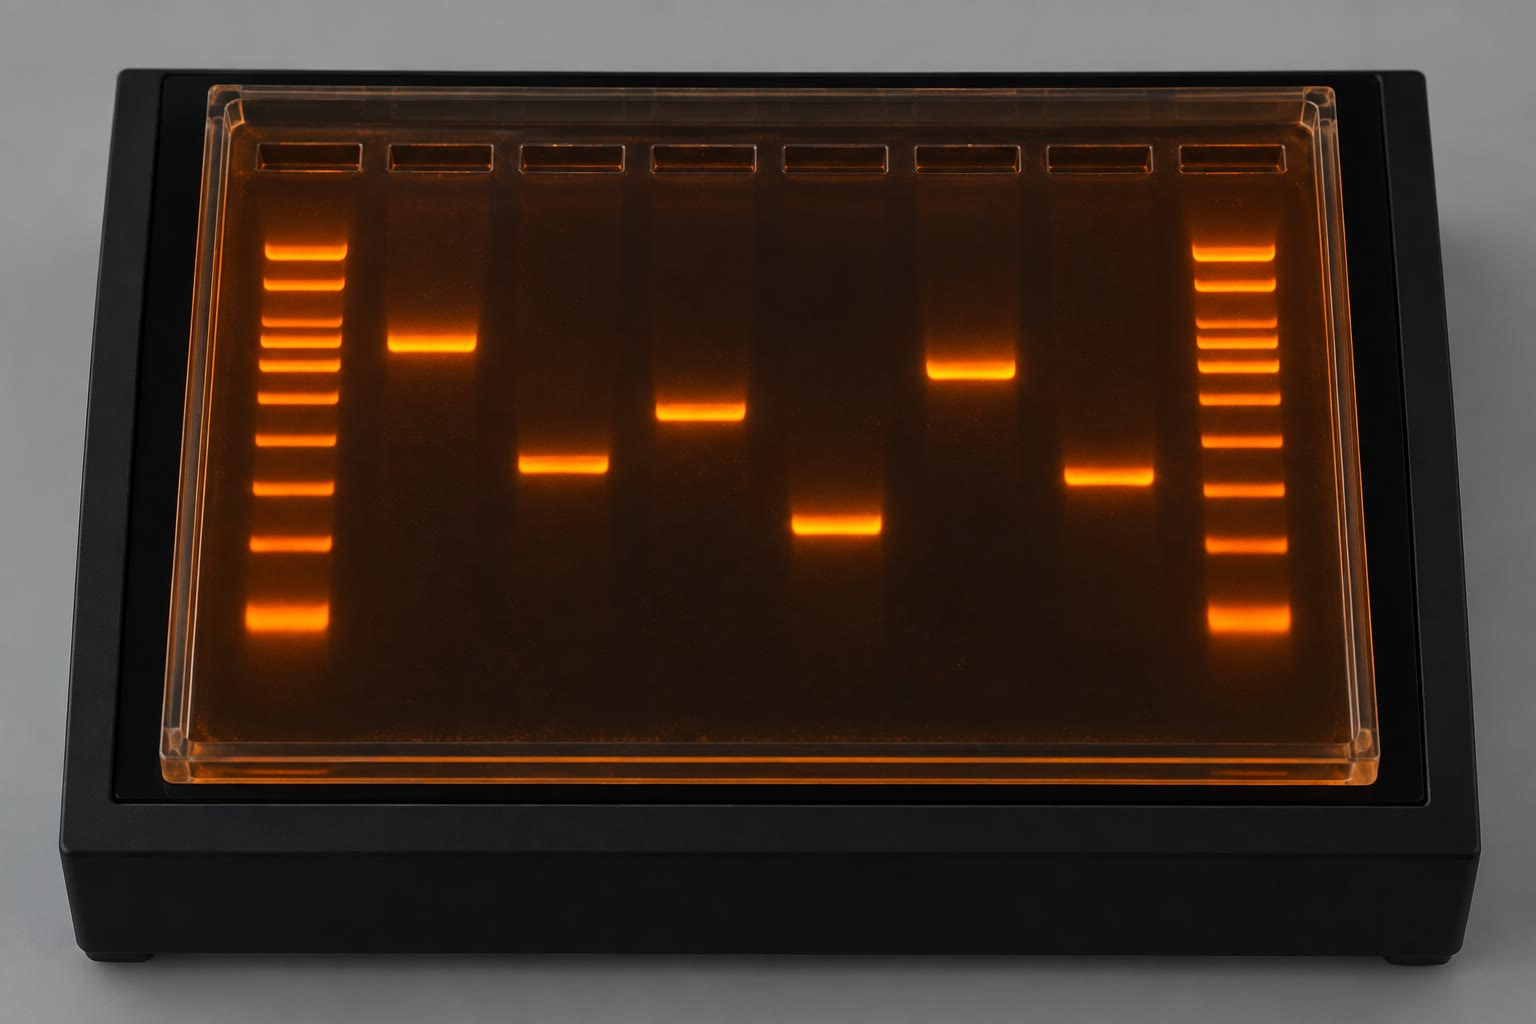
\includegraphics[width=0.56\linewidth]{images/book5/ai/b5-06-agarose-gel.jpg}

{\small Sebuah gel agarosa di bawah cahaya ultraungu: fragmen DNA bermigrasi
menuju anode dengan laju yang turun seiring panjangnya, sehingga tiap pitanya
adalah sekumpulan molekul berukuran satu, yang dibandingkan dengan tangga
ukuran yang telah diketahui pada jalur terluarnya.}
\end{omfigure}

\begin{definition}[Reaksi berantai polimerase]\label{def:b3:genetic-engineering:pcr}
\index{reaksi berantai polimerase}\index{primer}\index{PCR kuantitatif}
\emph{Reaksi berantai polimerase} (PCR) memperbanyak bentangan DNA pilihan di
antara dua \emph{primer} --- oligonukleotida sintetik sepanjang kira-kira dua
puluh basa yang komplementer dengan kedua untai pada ujung sasarannya ---
lewat daur tiga suhu: \qty{95}{\celsius} untuk memisahkan untainya,
\qtyrange{50}{65}{\celsius} agar primernya menempel, \qty{72}{\celsius} agar
polimerase tahan panas (Taq, dari bakteri sumber air panas \emph{Thermus
aquaticus}) memanjangkannya. Tiap daur melipatduakan cacah salinan segmen di
antara primernya, sehingga tiga puluh daur mengubah satu molekul menjadi
semiliar. \emph{PCR transkripsi balik} mula-mula menyalin RNA menjadi DNA
sehingga mengukur transkrip atau virus RNA; \emph{PCR kuantitatif} (qPCR)
mengikuti perbanyakannya secara waktu nyata dengan zat warna berpendar lalu
membaca kuantitas awalnya dari daur ketika isyaratnya melewati sebuah ambang.
\end{definition}

\begin{theorem}[Aritmetika perbanyakan]\label{thm:b3:genetic-engineering:pcr}
\index{daur ambang}
Dengan daya guna $E$ tiap daur ($E = 1$ bagi pelipatduaan sempurna), $N_{0}$
salinan awal menjadi
\[
N_{n} = N_{0}\,(1 + E)^{n}
\]
sesudah $n$ daur. Bila pendarannya melewati sebuah ambang tetap ketika
cacah salinannya mencapai $N_{T}$, \emph{\omterm{thm:b3:genetic-engineering:pcr}{daur ambangnya}} adalah
\[
C_{T} = \frac{\log N_{T} - \log N_{0}}{\log(1 + E)},
\]
yakni sebuah garis lurus dalam $\log N_{0}$ dengan kemiringan
$-1/\log(1+E)$: bagi $E = 1$, tiap kenaikan sepuluh kali lipat kuantitas
awalnya menurunkan $C_{T}$ sebesar $\log_{2} 10 = 3.32$ daur, dan dua contoh
yang \omterm{thm:b3:genetic-engineering:pcr}{daur ambangnya} berselisih $\Delta C_{T}$ berselisih salinan awal
sebesar faktor $(1 + E)^{\Delta C_{T}}$.
\end{theorem}
\begin{proof}
Tiap daur mengalikan cacah salinannya dengan $1 + E$, sehingga $N_{n}$
merupakan barisan geometrik. Menetapkan $N_{n} = N_{T}$ lalu menyelesaikannya
bagi $n$ memberi $C_{T}$; kemiringannya adalah koefisien $\log N_{0}$. Bagi
dua contoh, $C_{T,1} - C_{T,2} = (\log N_{0,2} - \log N_{0,1})/\log(1+E)$,
sehingga $N_{0,2}/N_{0,1} = (1+E)^{\Delta C_{T}}$.
\end{proof}

\begin{example}[Membaca sebuah pelat qPCR]\label{ex:b3:genetic-engineering:qpcr}
Sebuah uji RNA virus melewati ambangnya pada daur $22$ bagi seorang pasien
dan pada daur $32$ bagi pasien yang lain; dengan $E \approx 1$ yang pertama
mengusung virus $2^{10}
\approx 1000$ kali lebih banyak. Sebuah contoh berisi sepuluh salinan melewati
ambangnya kira-kira pada daur $37$ ketika ambangnya $10^{12}$ salinan ($\log_{2} 10^{11} =
36.5$); sekali jalan berisi $40$ daur karena itu mendeteksi beberapa molekul,
dan satu molekul cemaran dari amplikon sebelumnya pun terdeteksi, dan itulah
sebabnya laboratorium memisahkan ruang tempat PCR disiapkan dari ruang tempat
hasilnya ditangani.
\end{example}

\begin{omfigure}
\begin{tikzpicture}
\begin{axis}[
  width=0.7\linewidth, height=5.6cm,
  axis x line=bottom, axis y line=left,
  xmin=0, xmax=40, ymin=1, ymax=1e14, ymode=log,
  xlabel={daur}, ylabel={salinan},
  xlabel style={font=\small, at={(axis description cs:0.5,-0.12)}, anchor=north},
  ylabel style={font=\small},
  tick label style={font=\small}, xtick={0,10,20,30,40},
  clip=false,
]
\addplot[very thick, omDef, domain=0:40, samples=41] {1e7*2^x/(1+2^x/1e5)};
\addplot[very thick, omThm, domain=0:40, samples=41] {1e4*2^x/(1+2^x/1e8)};
\addplot[very thick, omMeth!70!black, domain=0:40, samples=41] {10*2^x/(1+2^x/1e11)};
\addplot[dashed, gray, domain=0:40, samples=2] {1e12};
\node[font=\scriptsize, gray, anchor=south west] at (axis cs:0.5,1.3e12) {ambang $N_{T}$};
\draw[gray] (axis cs:16.6,1) -- (axis cs:16.6,1e12); \draw[gray] (axis cs:26.6,1) -- (axis cs:26.6,1e12); \draw[gray] (axis cs:36.5,1) -- (axis cs:36.5,1e12);
\node[font=\scriptsize, anchor=south] at (axis cs:16.6,3e12) {$C_{T} = 16.6$}; \node[font=\scriptsize, anchor=south] at (axis cs:26.6,3e12) {$26.6$}; \node[font=\scriptsize, anchor=south] at (axis cs:36.5,3e12) {$36.5$};
\end{axis}
\end{tikzpicture}

{\small Kurva perbanyakan bagi $N_{0} = 10^{7}$ (biru), $10^{4}$ (merah),
dan $10$ salinan (hijau), $E = 1$, dengan dataran tinggi yang dipaksakan
pereaksinya. Selisih seribu kali lipat pada
$N_{0}$ menggeser \omterm{thm:b3:genetic-engineering:pcr}{daur ambangnya} sebesar $10$; dataran tingginya serupa
semua, dan itulah sebabnya hasil akhirnya tak mengatakan apa pun tentang
awalnya.}
\end{omfigure}

\section{Membuat protein}

\begin{definition}[Sistem ekspresi]\label{def:b3:genetic-engineering:expression}
\index{vektor ekspresi}\index{protein rekombinan}\index{antibodi monoklonal}
Sebuah \emph{\omterm{def:b3:genetic-engineering:tools}{vektor} ekspresi} menempatkan urutan penyandi yang telah diklon di
bawah promotor inangnya yang kuat dan terkendali (promotor \emph{lac} atau T7
pada \emph{E.~coli}, yang diimbas sebuah analog gula), dengan sebuah tapak
pengikat ribosom, sebuah terminator, dan kerap sebuah \emph{tanda} --- enam
histidina, sebuah protein kecil --- yang difusikan pada hasilnya demi
pemurnian pada sebuah kolom. Bakteri membuat beberapa gram tiap liter protein
sederhana (insulin, hormon pertumbuhan, enzim) tetapi tak dapat
mengglikosilasi atau melipat protein mamalia yang rumit; khamir menambahkan
gula jenisnya sendiri; sel serangga dan sel mamalia (sel ovarium hamster Cina
adalah baku industrinya) membuat antibodi dan faktor pembekuan yang terlipat
dan terglikosilasi seperti pada manusia. Sebuah \emph{antibodi monoklonal}
dibuat sebuah \emph{hibridoma} --- sel B penghasil antibodi yang difusikan
dengan sel mieloma yang baka (Köhler dan Milstein, 1975) --- atau, kini, dengan
mengklon gen antibodinya ke dalam galur ekspresi mamalia, dan di situ kerangka
mencitnya dapat diganti urutan manusia demi menghindari penolakan kekebalan
(\cref{ch:b3:adaptive-immunity}).
\end{definition}

\begin{example}[Insulin]\label{ex:b3:genetic-engineering:insulin}
Insulin manusia terdiri atas dua rantai, A (21 residu) dan B (30), yang
disambungkan ikatan disulfida, dan dipotong di dalam sel $\beta$ dari satu
pendahulu proinsulin. Proses pertamanya mengekspresikan kedua rantai itu
terpisah di dalam \emph{E.~coli}, masing-masing difusikan pada
$\beta$-galaktosidase, lalu memotongnya secara kimia dan menyambungkannya di
luar sel; proses yang kemudian mengekspresikan proinsulin lalu memotongnya
dengan enzim yang dipakai pankreas. Sejak tahun 1996 urutannya sendiri telah
diubah: menukar atau menambahkan satu dua residu memberi analog yang terurai
lebih cepat (bagi sekali makan) atau mengendap di tempat suntikan lalu
dilepaskan sepanjang sehari. Sebuah protein yang dahulu menuntut delapan ton
kelenjar tiap kilogram kini dibuat di dalam fermenter, identik dengan protein
manusia atau lebih baik daripadanya.
\end{example}

\section{Organisme transgenik}

\begin{definition}[Transgenesis dan penyasaran gen]\label{def:b3:genetic-engineering:transgenic}
\index{organisme transgenik}\index{mikroinjeksi}\index{penidakaktifan gen}%
\index{sel punca embrio}\index{penyasaran gen}
Sebuah organisme \emph{transgenik} mengusung gen yang dimasukkan ke dalam
garis nutfahnya, sehingga tiap selnya memilikinya dan gen itu diwariskan. Pada
mencit rute klasiknya adalah \emph{mikroinjeksi} DNA-nya ke dalam salah satu
pronukleus telur yang telah dibuahi (Gordon dan Ruddle, 1980), yang terpadu
pada tapak acak di dalam sebagian embrionya; Palmiter dan Brinster (1982)
membuat mencit berukuran dua kali normal dengan menyuntikkan gen hormon
pertumbuhan tikus di belakang promotor metalotionein. \emph{Penyasaran gen}
justru mengganti atau merusak gen pilihan: sebuah konstruk berlengan panjang
yang homolog dengan sasarannya dimasukkan ke dalam \emph{sel punca embrio},
sel langka yang di dalamnya \omterm{def:b3:dna-repair:dsb}{rekombinasi homolog} telah menaruhnya di tempat
yang benar lalu dipilih dan disuntikkan ke dalam sebuah blastosista, dan
mencit kimeris yang dihasilkannya meneruskan gen yang telah diubah itu
(Capecchi, Smithies, dan Evans, dasawarsa 1980-an). Sebuah
\emph{penidakaktifan} kehilangan gennya; sebuah \emph{penyisipan} mengusung
versi yang telah diubah; sebuah alel \emph{bersyarat}, yang diapit tapak loxP,
dihapus hanya di tempat dan pada waktu Cre diekspresikan
(\cref{ch:b3:dna-repair}). Sekitar sepuluh ribu gen mencit telah
dinonaktifkan, dan bagi sebagian besarnya fenotipenya menjadi petunjuk pertama
tentang apa yang dikerjakan gen itu.
\end{definition}

\begin{omfigure}
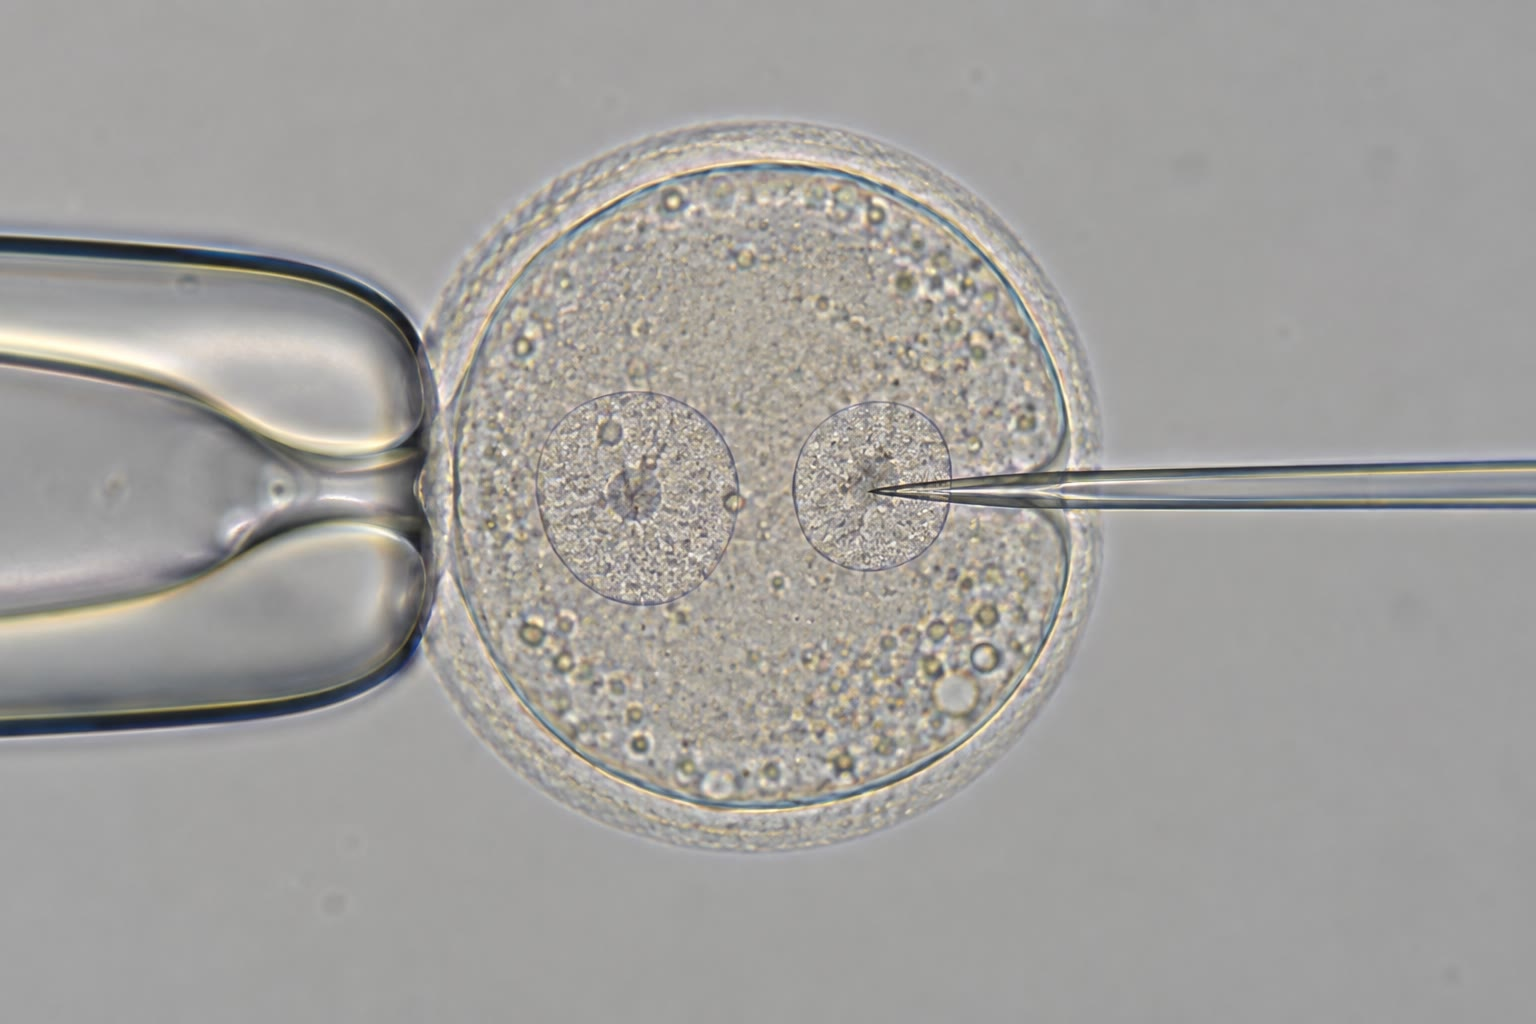
\includegraphics[width=0.46\linewidth]{images/book5/ai/b5-06-microinjection.jpg}\hspace{0.04\linewidth}
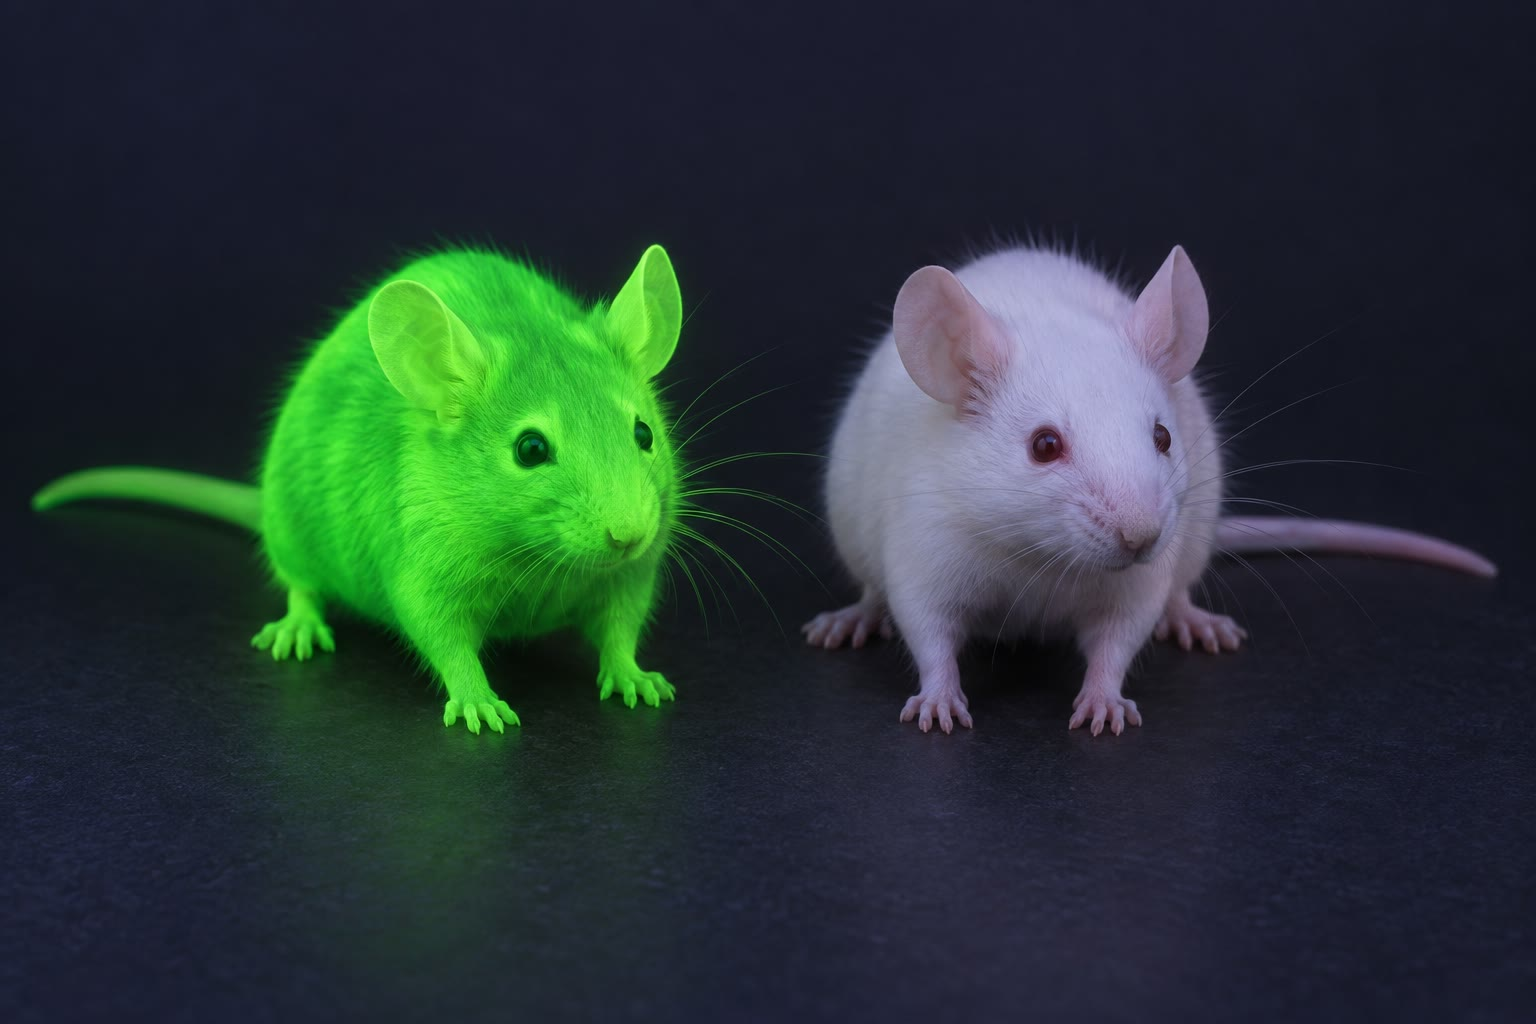
\includegraphics[width=0.46\linewidth]{images/book5/ai/b5-06-gfp-mouse.jpg}

{\small Kiri: sebuah telur mencit yang telah dibuahi ditahan dengan isapan
sementara sebuah jarum kaca menyuntikkan DNA ke dalam salah satu pronukleusnya.
Kanan: seekor mencit \omterm{def:b3:genetic-engineering:transgenic}{transgenik} yang mengekspresikan protein berpendar hijau
milik ubur-ubur di setiap selnya, di samping saudara seperindukannya yang
biasa, di bawah cahaya ultraungu.}
\end{omfigure}

\begin{definition}[Tumbuhan transgenik]\label{def:b3:genetic-engineering:plants}
\index{Agrobacterium}\index{T-DNA}\index{tanaman termodifikasi genetik}
Tumbuhan ditransformasi oleh \emph{Agrobacterium tumefaciens}, bakteri tanah
yang secara alami menyisipkan sepotong \omterm{def:b3:genetic-engineering:tools}{plasmid} pengimbas tumornya, yaitu
\emph{T-DNA}, ke dalam genom tumbuhan yang terluka agar tumbuhan itu
menumbuhkan puru lalu menyuapi bakterinya. Mengganti gen milik T-DNA itu
sendiri dengan gen pilihan mana pun, di antara urutan batas yang dikenali
bakterinya, mengubah patogennya menjadi sebuah \omterm{def:b3:genetic-engineering:tools}{vektor}; sel yang telah
ditransformasi dipilih lalu diregenerasi menjadi tumbuhan utuh, yang dapat
dikerjakan setiap sel tumbuhan. Spesies yang tak diinfeksi bakteri itu (serealia,
untuk waktu yang lama) ditransformasi dengan menembakkan butiran emas berlapis
DNA ke dalam jaringannya. \emph{Tanaman termodifikasi genetik} yang ditanam
secara luas mengusung gen toksin bakteri (\emph{Bt}) yang melawan larva
serangga, atau enzim bakteri yang memberi toleransi terhadap herbisida, atau
keduanya; adapun \emph{Padi Emas} mengusung dua gen jalur karotenoid (fitoena
sintase tumbuhan dan sebuah desaturase bakteri) sehingga endospermanya membuat
$\beta$-karotena, pendahulu vitamin~A, yang kekurangannya membutakan dan
membunuh beberapa ratus ribu anak tiap tahun.
\end{definition}

\begin{omfigure}
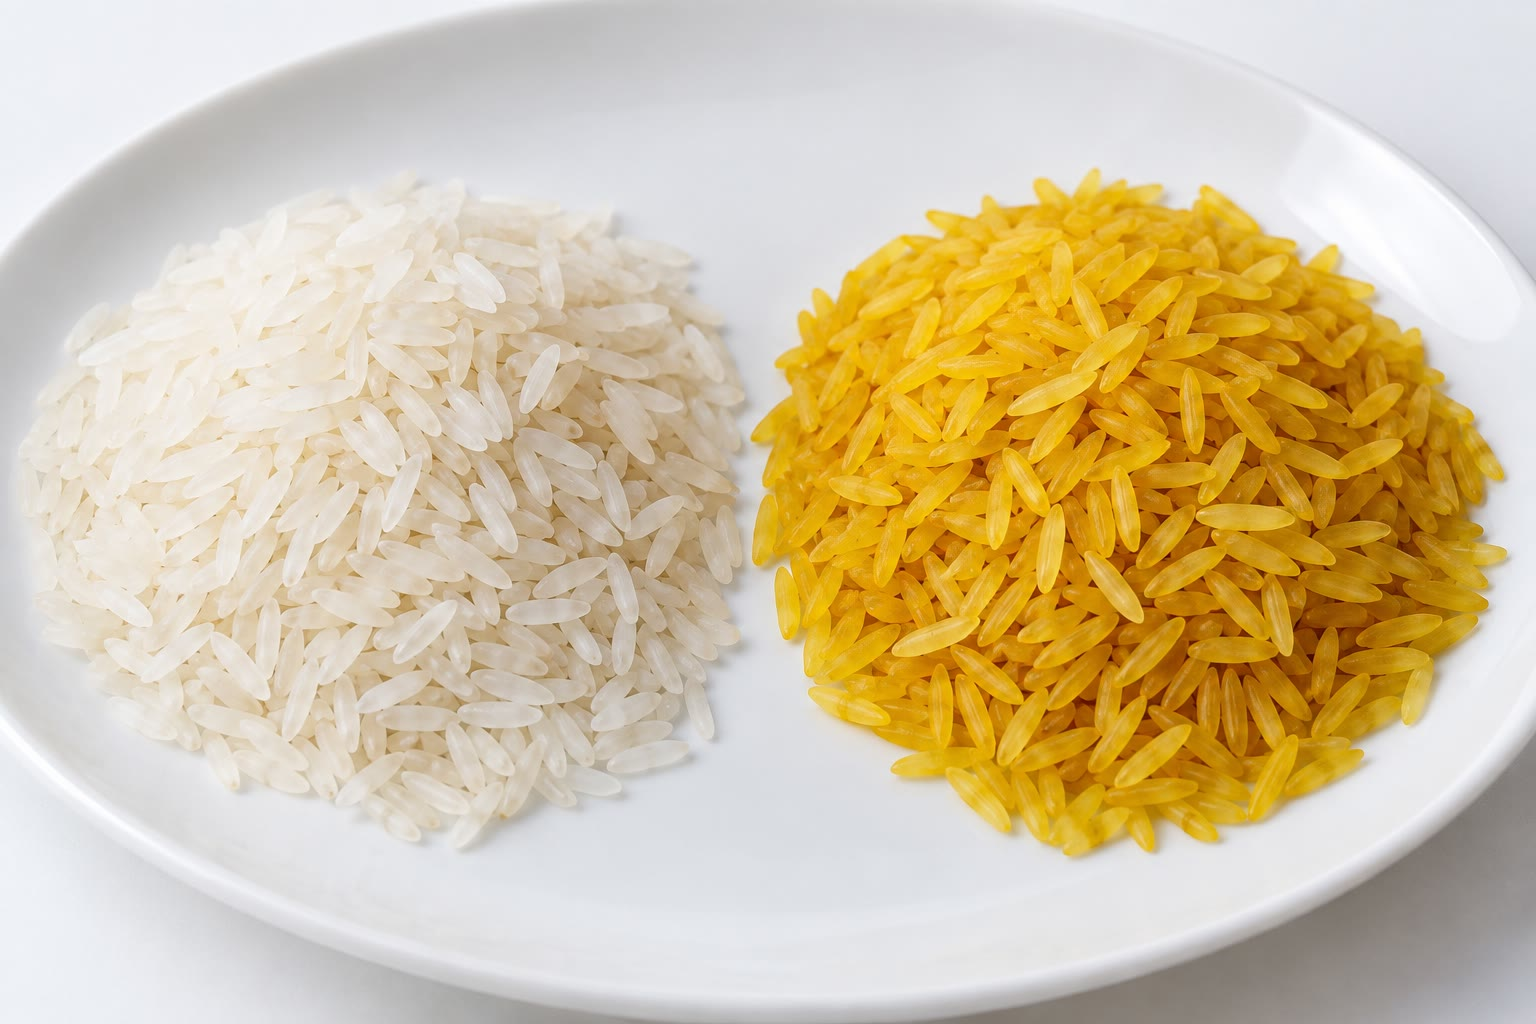
\includegraphics[width=0.46\linewidth]{images/book5/ai/b5-06-golden-rice.jpg}\hspace{0.04\linewidth}
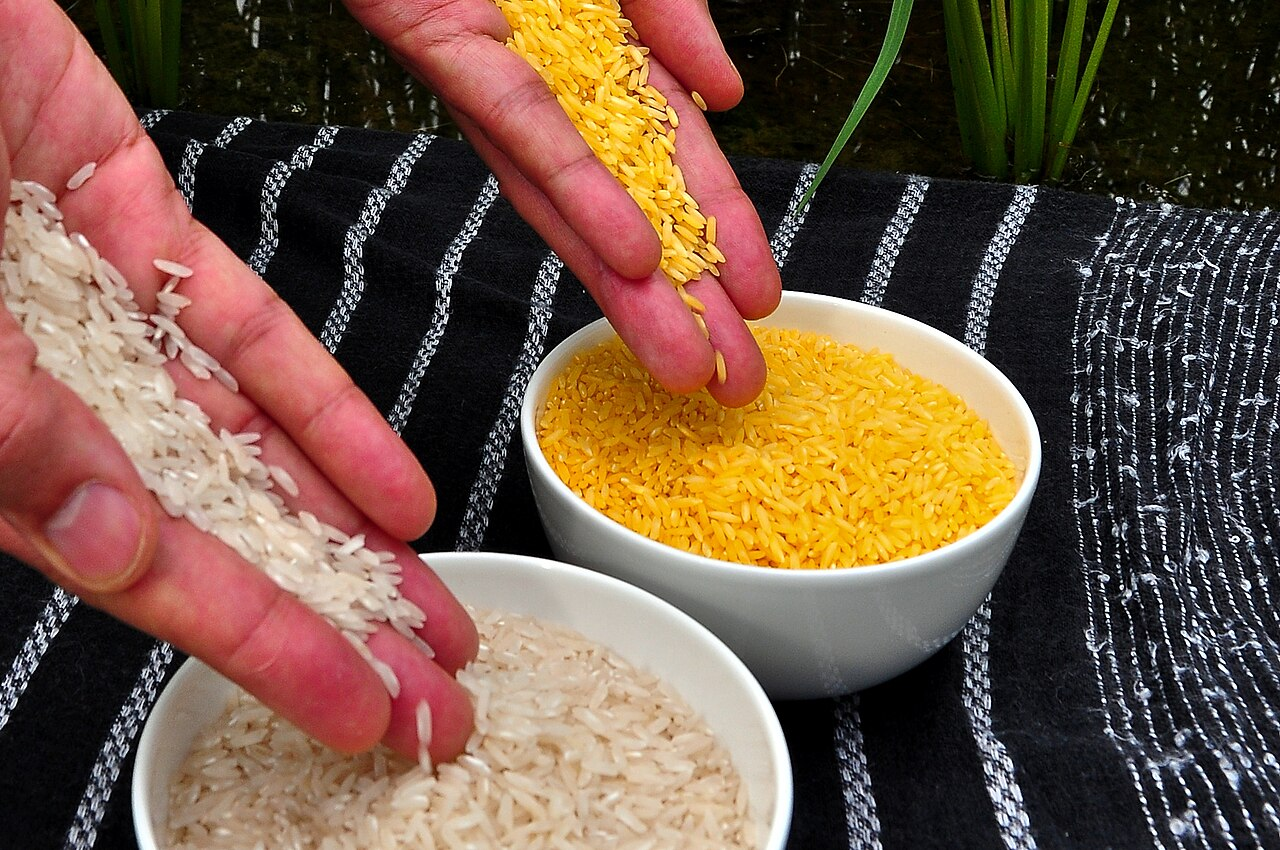
\includegraphics[width=0.46\linewidth]{images/book5/golden-rice-irri.jpg}

{\small Padi biasa dan Padi Emas. Butir yang kuning membuat
$\beta$-karotena di dalam endospermanya dari dua gen tambahan jalur
karotenoidnya. Kanan: kedua padi itu dibandingkan di
International Rice Research Institute (IRRI, CC~BY~2.0).}
\end{omfigure}

\begin{remark}[Perdebatannya]\label{rem:b3:genetic-engineering:gmo}
Tiga puluh tahun penanaman pada ratusan juta hektar, dan setiap tinjauan
sistematis oleh akademi ilmu pengetahuan, tidak menemukan pengaruh kesehatan
tanaman \omterm{def:b3:genetic-engineering:transgenic}{transgenik} yang telah disetujui yang berbeda dari tanaman padanannya
yang konvensional; transgennya hanya satu gen di antara empat puluh ribu, dan
protein yang dibuatnya diuji sebagaimana zat tambahan pangan mana pun diuji.
Pertanyaan yang sungguhan bersifat ekologis dan ekonomis: menyebarnya
kekebalan pada hama dan gulma di bawah seleksi yang seragam, aliran gen ke
kerabat liar, memusatnya pasar benih, dan siapa yang diuntungkan. Itulah
pertanyaan yang ditimbulkan teknologi pertanian yang perkasa mana pun, dan
jawabannya bergantung pada sifat dan latarnya, bukan pada cara gennya
dipindahkan.
\end{remark}

\section{Menyunting genom}

\begin{definition}[CRISPR--Cas9]\label{def:b3:genetic-engineering:crispr}
\index{CRISPR}\index{Cas9}\index{RNA pemandu}\index{PAM}\index{penyuntingan genom}
Bakteri menyimpan fragmen genom fag yang telah menginfeksi moyangnya di dalam
sebuah larik ulangan (\emph{CRISPR}), mentranskripsinya menjadi RNA pemandu
yang pendek, lalu memakainya untuk mengarahkan sebuah nuklease agar memotong
DNA mana pun yang cocok dan masuk ke dalam selnya: sebuah sistem kekebalan
adaptif dengan ingatan genetik. Pada \emph{Streptococcus pyogenes}
nukleasenya adalah protein tunggal \emph{Cas9}, yang mengikat sebuah RNA
pemandu dan sebuah RNA kecil kedua, menelusuri DNA untuk mencari \emph{\omterm{def:b3:bioinformatics:motif}{motif}
bersebelahan protospacer} berbasa tiga (PAM, 5$'$-NGG), membuka pilinan DNA di
sebelahnya, dan, bila kedua puluh basa di samping PAM berpasangan dengan
pemandunya, memotong kedua untai pada jarak tiga basa dari PAM. Jinek,
Charpentier, Doudna, dan rekan (2012) memfusikan kedua RNA itu menjadi satu
\emph{RNA pemandu tunggal} lalu menunjukkan bahwa Cas9 dengan pemandu berurutan
pilihan mana pun memotong DNA pada urutan itu di dalam tabung reaksi; dalam
setahun pasangan itu terbukti bekerja di dalam sel manusia, mencit, ikan zebra,
tumbuhan, dan khamir. \emph{Penyuntingan genom} adalah apa yang dikerjakan sel
dengan potongan itu: penyambungan ujung meninggalkan sisipan atau delesi kecil
yang merusak gennya (sebuah penidakaktifan dalam satu langkah, pada organisme
mana pun, dalam hitungan minggu), dan \omterm{def:b3:dna-repair:dsb}{rekombinasi homolog} dengan cetakan yang
dipasok menuliskan urutan pilihan ke dalamnya.
\end{definition}

\begin{omfigure}
\begin{tikzpicture}[every node/.style={font=\scriptsize}, >=stealth]
  % Cas9 outline (drawn first so labels stay on top)
  \draw[thick, omExo, fill=omExo!15] (5.9,1.1) ellipse (2.6 and 1.6);
  \node[omExo!60!black] at (7.7,2.3) {Cas9};
  % target DNA
  \draw[very thick, omDef] (0,0.3) -- (11,0.3); \draw[very thick, omDef] (0,-0.1) -- (11,-0.1);
  % PAM
  \fill[omProp!60] (7.2,-0.2) rectangle (7.9,0.4); \node[below] at (7.55,-0.25) {PAM (NGG)};
  % protospacer
  \draw[omThm, very thick] (4.2,0.5) -- (7.15,0.5); \node[above] at (5.7,0.55) {sasaran 20 basa, berpasangan dengan pemandunya};
  % guide RNA
  \draw[very thick, omMeth!70!black] (4.2,0.3) .. controls (4.2,1.6) and (5.0,1.9) .. (5.4,1.9) -- (6.6,1.9) .. controls (7.0,1.9) and (7.2,2.5) .. (6.8,2.8) .. controls (6.3,3.1) and (5.8,2.7) .. (6.1,2.4);
  \node[left, omMeth!70!black, align=right] at (3.2,2.2) {RNA pemandu tunggal:\\20 basa pilihan\\+ jepit rambut pengikat Cas9};
  % cut
  \draw[omThm, very thick, ->] (6.25,-0.7) -- (6.25,0.35); \node[omThm, below] at (6.25,-0.7) {putus untai ganda, 3 basa dari PAM};
  % outcomes
  \draw[->, thick] (2.0,-1.3) -- (2.0,-1.9); \node[below, align=center] at (2.0,-1.9) {penyambungan ujung:\\sisipan atau delesi kecil\\$\Rightarrow$ geser kerangka, gen mati};
  \draw[->, thick] (10.0,-1.3) -- (10.0,-1.9); \node[below, align=center] at (10.0,-1.9) {rekombinasi dengan\\cetakan yang dipasok\\$\Rightarrow$ perubahan yang saksama};
\end{tikzpicture}

{\small \omterm{def:b3:genetic-engineering:crispr}{Cas9} dan pemandunya. Proteinnya mengikat sebuah \omterm{def:b3:genetic-engineering:crispr}{PAM}, membuka pilinan
DNA di sebelahnya, lalu memotong bila kedua puluh basanya berpasangan dengan
\omterm{def:b3:genetic-engineering:crispr}{RNA pemandunya}. Putusnya diperbaiki entah oleh penyambungan ujung, yang
merusak gennya, entah oleh rekombinasi dengan sebuah cetakan, yang menulis
ulang gennya.}
\end{omfigure}

\begin{proposition}[Menyunting tanpa memutus]\label{prop:b3:genetic-engineering:editors}
\index{penyunting basa}\index{penyunting prima}\index{luar sasaran}
Memotong kedua untai adalah suntingan yang paling kasar: hasil penyambungan
ujungnya acak, dan sebuah putus di tempat lain --- tapak \emph{\omterm{prop:b3:genetic-engineering:editors}{luar sasaran}}
yang berbeda dari pemandunya pada beberapa kedudukan, yang masih ditoleransi
\omterm{def:b3:genetic-engineering:crispr}{Cas9} --- adalah mutasi yang tak diminta siapa pun. \omterm{def:b3:genetic-engineering:crispr}{Cas9} yang satu domain
nukleasenya dinonaktifkan menakik satu untai saja; bila keduanya dinonaktifkan
ia sekadar mengikat, dan dapat mengusung enzim lain ke sebuah urutan.
\emph{\omterm{prop:b3:genetic-engineering:editors}{Penyunting basa}} memfusikan \omterm{def:b3:genetic-engineering:crispr}{Cas9} penakik pada sebuah deaminase yang
mengubah C menjadi U (terbaca sebagai T) atau A menjadi I (terbaca sebagai G)
pada untai yang terbuka pilinannya, sehingga mengubah satu basa tanpa putus
dan tanpa cetakan; \emph{\omterm{prop:b3:genetic-engineering:editors}{penyunting prima}} mengusung sebuah transkriptase
balik dan sebuah pemandu yang diperpanjang dengan urutan yang diinginkan, lalu
menyalin urutan itu ke dalam untai yang tertakik, sehingga membolehkan
substitusi apa pun serta sisipan dan delesi kecil. Keaktifan \omterm{prop:b3:genetic-engineering:editors}{luar sasarannya}
dikurangi dengan varian \omterm{def:b3:genetic-engineering:crispr}{Cas9} berkesetiaan tinggi hasil rekayasa, dengan
mengantarkan enzimnya sejenak sebagai protein alih-alih sebagai gen, dan
dengan memilih pemandu yang kerabat genomik terdekatnya berbeda pada beberapa
kedudukan; keaktifan itu diukur dengan mengurutkan tapak yang diramalkan, dan
dengan metode tak bias yang menangkap setiap putus di dalam genomnya.
\end{proposition}

\begin{example}[Sebuah penyembuhan]\label{ex:b3:genetic-engineering:sickle}
Penyakit sel sabit adalah perubahan satu basa pada $\beta$-globin. Hemoglobin
janin, yang dibuat dari $\gamma$-globin, dapat menggantikannya, tetapi gen
$\gamma$-nya dimatikan sesudah lahir oleh penekan BCL11A.
Terapi \omterm{def:b3:genetic-engineering:crispr}{CRISPR} pertama yang disetujui (2023) mengambil sel punca darah pasien
itu sendiri, memotong penguat eritroid \emph{BCL11A} dengan \omterm{def:b3:genetic-engineering:crispr}{Cas9} sehingga
penyambungan ujung melumpuhkannya di sebagian besar selnya, lalu mengembalikan
selnya sesudah sumsum pasiennya dikosongkan: sel darah merah yang dibuatnya
kaya hemoglobin janin, tidak menyabit, dan krisisnya berhenti. Suntingannya
bersifat somatik --- garis nutfahnya tak tersentuh dan perubahannya tak
diwariskan --- dan suntingan itu memakai hasil yang ``kasar'', yaitu
perusakan, di tempat perusakan justru yang diinginkan.
\end{example}

\begin{theorem}[Penyebaran super-Mendel sebuah penggerak gen]\label{thm:b3:genetic-engineering:drive}
\index{penggerak gen}
Sebuah \emph{\omterm{thm:b3:genetic-engineering:drive}{penggerak gen}} adalah konstruk yang menyandikan \omterm{def:b3:genetic-engineering:crispr}{Cas9} dan sebuah
pemandu yang memotong alel tipe liar pada lokusnya sendiri di dalam sebuah
heterozigot; perbaikan lewat rekombinasi menyalin penggeraknya ke dalam
kromosom yang terpotong, sehingga sebagian $c$ gamet heterozigot itu mengusung
penggeraknya alih-alih separuh menurut Mendel. Bila penggeraknya berfrekuensi
$p$ di dalam populasi besar yang kawin secara acak dan tanpa ongkos kebugaran,
frekuensinya pada generasi berikutnya adalah
\[
p' = p + c\,p\,(1 - p),
\]
sehingga penggeraknya menyebar dari kelangkaan dengan laju sebanding dengan
$c$, dan mencapai separuh populasinya dalam kira-kira
$\ln(1/p_{0})/\ln(1 + c)$ generasi dari frekuensi awal $p_{0}$.
\end{theorem}
\begin{proof}
Kawin acak memberi homozigot bagi penggeraknya pada frekuensi $p^{2}$,
heterozigot pada $2p(1-p)$, dan homozigot tipe liar pada $(1-p)^{2}$.
Homozigotnya meneruskan penggeraknya ke seluruh gametnya, heterozigotnya ke
bagian $(1 + c)/2$ (separuh menurut Mendel, ditambah $c$ kali separuh tipe
liar yang terkonversi), dan tipe liarnya tidak sama sekali. Jadi $p' = p^{2} + 2p(1-p)(1+c)/2
= p^{2} + p(1-p) + c\,p(1-p) = p + c\,p(1-p)$. Bagi $p$ kecil hal ini menjadi
$p' \approx (1+c)p$, yakni pertumbuhan geometrik berasio $1 + c$, yang mencapai
$1/2$ dari $p_{0}$ sesudah kira-kira $\ln(1/2p_{0})/\ln(1+c)$ generasi; suku
logistiknya hanya memperlambatnya menjelang akhir.
\end{proof}

\begin{omfigure}
\begin{tikzpicture}
\begin{axis}[
  width=0.7\linewidth, height=5.6cm,
  axis x line=bottom, axis y line=left,
  xmin=0, xmax=20, ymin=0, ymax=1.05,
  xlabel={generasi}, ylabel={frekuensi penggerak $p$},
  xlabel style={font=\small, at={(axis description cs:0.5,-0.12)}, anchor=north},
  ylabel style={font=\small},
  tick label style={font=\small}, xtick={0,5,10,15,20}, ytick={0,0.5,1},
  clip=false,
]
\addplot[very thick, omThm, mark=*, mark size=1.2pt] coordinates {(0,0.01) (1,0.0189) (2,0.0356) (3,0.0665) (4,0.1224) (5,0.2191) (6,0.3731) (7,0.5836) (8,0.8023) (9,0.9451) (10,0.9918) (11,0.9991) (12,1.0) (13,1.0) (14,1.0) (15,1.0) (16,1.0) (17,1.0) (18,1.0) (19,1.0) (20,1.0)};
\addplot[very thick, omDef, mark=*, mark size=1.2pt] coordinates {(0,0.01) (1,0.015) (2,0.0223) (3,0.0332) (4,0.0493) (5,0.0727) (6,0.1064) (7,0.154) (8,0.2191) (9,0.3047) (10,0.4106) (11,0.5316) (12,0.6561) (13,0.769) (14,0.8578) (15,0.9188) (16,0.9561) (17,0.9771) (18,0.9883) (19,0.9941) (20,0.997)};
\addplot[very thick, gray, dashed, domain=0:20, samples=2] {0.01};
\node[font=\scriptsize, omThm, anchor=south east] at (axis cs:6.5,0.62) {$c = 0.9$};
\node[font=\scriptsize, omDef, anchor=north west] at (axis cs:12.5,0.62) {$c = 0.5$};
\node[font=\scriptsize, gray, anchor=south west] at (axis cs:12,0.02) {Mendel, $c = 0$: tetap pada $p_{0}$};
\end{axis}
\end{tikzpicture}

{\small Sebuah \omterm{thm:b3:genetic-engineering:drive}{penggerak gen} yang dilepaskan pada satu persen, dengan daya
guna konversi $0.9$ atau $0.5$ dan tanpa ongkos kebugaran. Alel Mendel tanpa
keunggulan akan tetap pada satu persen; penggeraknya menguasai populasinya
dalam sepuluh atau dua puluh generasi.}
\end{omfigure}

\begin{remark}[Apa yang boleh disunting]\label{rem:b3:genetic-engineering:ethics}
Menyunting sel somatik seorang pasien yang menyetujuinya adalah pengobatan,
yang dinilai seperti perawatan mana pun menurut risiko dan manfaatnya.
Menyunting garis nutfah --- sebuah embrio, yang setiap keturunannya akan
mengusung perubahan itu --- berbeda jenisnya: orang yang terkena tak dapat
menyetujuinya, perubahannya diwariskan, dan hasil \omterm{prop:b3:genetic-engineering:editors}{luar sasaran} serta mozaik
tekniknya belum terkendali; sesudah seorang ilmuwan Cina mengumumkan pada
tahun 2018 bahwa ia telah melakukannya pada sepasang bayi kembar, akademi ilmu
pengetahuan sebagian besar negara menyerukan moratorium dan beberapa negara
menjadikannya kejahatan. Sebuah \omterm{thm:b3:genetic-engineering:drive}{penggerak gen} yang dilepaskan ke dalam populasi
liar adalah keputusan yang diambil bagi semua orang di hilirnya, dan itulah
sebabnya usulan bidang ini sendiri bagi pembasmian nyamuk malaria menggandengkan
penggeraknya pada pengaman --- penggerak pembalik, rancangan yang membatasi
diri --- dan pada persetujuan publik di negara yang bersangkutan.
\end{remark}

\section{Latihan}

\begin{exercise}[$\star$]\label{exo:b3:genetic-engineering:1}
Sebutkanlah ketiga komponen yang harus dimiliki sebuah \omterm{def:b3:genetic-engineering:tools}{plasmid} pengklonan lalu
jelaskan tujuan masing-masing.
\end{exercise}

\begin{exercise}[$\star$]\label{exo:b3:genetic-engineering:2}
EcoRI mengenali GAATTC. Berapa sering tapaknya muncul, rata-rata, di dalam DNA
acak, dan berapa fragmen yang dibuatnya dari genom \emph{E.~coli} \qty{4.6}{Mb}?
Mengapa cacah yang sesungguhnya agak berbeda?
\end{exercise}

\begin{exercise}[$\star$]\label{exo:b3:genetic-engineering:3}
Nyatakanlah ketiga langkah suhu sebuah daur PCR dan apa yang terjadi pada
masing-masing. Mengapa polimerasenya harus tahan panas?
\end{exercise}

\begin{exercise}[$\star$]\label{exo:b3:genetic-engineering:4}
Apa yang dibutuhkan \omterm{def:b3:genetic-engineering:crispr}{Cas9} agar dapat memotong sebuah urutan tertentu, dan dua
hasil apa yang dapat menyusul potongan itu?
\end{exercise}

\begin{exercise}[$\star\star$]\label{exo:b3:genetic-engineering:5}
Sebuah PCR berjalan $35$ daur pada daya guna $E = 0.9$ dari $50$ salinan.
Berapa salinan yang dihasilkannya? Sebuah qPCR atas dua contoh memberi
$C_{T} = 18.2$ dan $25.5$; dengan $E = 0.95$, berapa nisbah kuantitas awalnya?
\end{exercise}

\begin{exercise}[$\star\star$]\label{exo:b3:genetic-engineering:6}
Mengapa pustaka cDNA, dan bukan pustaka genom, yang dipakai untuk
mengekspresikan protein manusia di dalam bakteri? Sebutkanlah dua rintangan
lain bagi pembuatan protein manusia di dalam \emph{E.~coli} lalu katakan cara
mengatasi masing-masing.
\end{exercise}

\begin{exercise}[$\star\star$]\label{exo:b3:genetic-engineering:7}
Seekor mencit dengan gen yang dinonaktifkan dibuat lewat \omterm{def:b3:genetic-engineering:transgenic}{penyasaran gen} pada
\omterm{def:b3:genetic-engineering:transgenic}{sel punca embrio}. Jelaskanlah mengapa mencit pertama yang lahir adalah sebuah
kimera, mengapa ia harus dikawinkan, dan berapa bagian cucu seekor kimera
yang separuh garis nutfahnya tersasar yang menjadi homozigot tanpa gen itu
bila cucu heterozigotnya disilangkan satu sama lain.
\end{exercise}

\begin{exercise}[$\star\star$]\label{exo:b3:genetic-engineering:8}
Sebuah \omterm{def:b3:genetic-engineering:crispr}{RNA pemandu} berbasa 20 dengan \omterm{def:b3:genetic-engineering:crispr}{PAM} berupa NGG dipilih. Berapa tapak di
dalam genom berisi $3.2\times 10^{9}$ bp (kedua untainya) yang cocok persis
dengan pemandunya secara kebetulan? Berapa yang cocok dengan paling banyak dua
ketakcocokan, bila \omterm{def:b3:genetic-engineering:crispr}{Cas9} mentoleransinya? (Hitunglah urutan yang berada dalam
dua ketakcocokan sebagai $1 + 3\binom{20}{1} +
9\binom{20}{2}$.)
\end{exercise}

\begin{exercise}[$\star\star$]\label{exo:b3:genetic-engineering:9}
Dengan \cref{thm:b3:genetic-engineering:drive}, hitunglah frekuensi sebuah
penggerak dengan $c = 0.8$ sesudah tiga generasi dari $p_{0} = 0.05$, lalu
taksirlah cacah generasi untuk mencapai $0.5$.
\end{exercise}

\begin{exercise}[$\star\star\star$]\label{exo:b3:genetic-engineering:10}
Terapi sel sabit merusak sebuah penguat alih-alih membetulkan mutasi
$\beta$-globinnya. Berikanlah dua alasan mengapa perusakan lewat penyambungan
ujung dipilih daripada pembetulan lewat \omterm{def:b3:dna-repair:dsb}{rekombinasi homolog} pada sel punca
darah, dan satu kelemahannya.
\end{exercise}

\begin{exercise}[$\star\star\star$]\label{exo:b3:genetic-engineering:11}
Sebuah \omterm{thm:b3:genetic-engineering:drive}{penggerak gen} melawan nyamuk mengusung ongkos kebugaran $s$ pada
homozigotnya. Ubahlah rekursinya agar memuat seleksi terhadap homozigot
penggeraknya lalu carilah syarat pada $c$ dan $s$ agar penggeraknya menyebar
dari kelangkaan. Lalu jelaskanlah mengapa alel kekebalan --- hasil penyambungan
ujung pada sasarannya yang tak lagi dikenali pemandunya --- menjadi rintangan
utama dalam praktiknya.
\end{exercise}

\begin{exercise}[$\star\star\star$]\label{exo:b3:genetic-engineering:12}
Kemukakanlah, dengan mekanisme bab ini dan
\cref{ch:b3:dna-repair}, mengapa penyuntingan garis nutfah embrio manusia
belum dapat menjamin hasil yang dituju pada tiap selnya, dan bukti apa yang
dibutuhkan sebelum seorang yang berakal sehat dapat menganggapnya aman.
\end{exercise}

\section{Soal: Dari Sebuah Gen ke Sebuah Obat dan Sebuah Tanaman}

\begin{problem}[{Soal akhir pekan --- sebuah gen yang diklon dengan aritmetika
tapak restriksi dan transformasi, sebuah virus yang dicacah dengan qPCR,
sebuah hormon yang diproduksi berton-ton di dalam fermenter, sebuah genom yang
disunting dengan luar sasarannya dicacah, dan sebuah penggerak gen yang
ditakar waktunya, berakhir pada salinan virus di dalam sebuah contoh, volume
fermenter tahunan bagi insulin dunia, dan cacah generasi yang dibutuhkan sebuah penggerak}]
\label{pb:b3:genetic-engineering:1}
Data: sebuah gen \qty{1.5}{kb}; sebuah tapak restriksi berbasa enam; sebuah
\omterm{def:b3:genetic-engineering:tools}{plasmid} \qty{4}{kb}; daya guna transformasi $2\times 10^{7}$ koloni tiap
mikrogram \omterm{def:b3:genetic-engineering:tools}{plasmid}; ligasinya memberi \qty{10}{\%} \omterm{def:b3:genetic-engineering:tools}{plasmid} sebuah
sisipan. Daya guna qPCR $E = 1$, ambangnya $N_{T} = 10^{12}$. Insulin:
\qty{5.8}{kDa}, seorang pasien memakai $40$ satuan tiap hari, satu satuan
sebesar \qty{35}{\micro g}; $10^{7}$ pasien; sebuah fermenter menghasilkan
\qty{2}{g/L} produk tiap gelombang, sepuluh gelombang tiap tahun. Genom $3.2\times
10^{9}$ bp. Konversi penggeraknya $c = 0.9$, dilepas pada $p_{0} = 0.001$.

\medskip
\noindent\textbf{Bagian I --- Pengklonan.}
\begin{enumerate}
  \item Berapa sering sebuah tapak berbasa enam tertentu muncul di dalam DNA
        acak? Berapa peluang bahwa gen \qty{1.5}{kb} itu tak memuat
        tapak semacam itu, sehingga enzimnya dapat dipakai mengklonnya utuh?
  \item Bila gennya memang memuat sebuah tapak, bagaimana Anda akan tetap
        mengklonnya? (Dua cara.)
  \item \qty{100}{ng} \omterm{def:b3:genetic-engineering:tools}{plasmid} yang telah diligasi ditransformasikan. Berapa
        koloninya, dan berapa yang membawa sisipannya?
  \item Penapisan biru--putih dipakai. Berapa bagian koloninya yang
        putih, dan berapa koloni putih yang harus dipungut agar berpeluang
        \qty{99}{\%} bahwa sedikitnya satu membawa gennya pada
        orientasi yang benar (separuh sisipannya)?
  \item \omterm{def:b3:genetic-engineering:tools}{Plasmid} rekombinannya \qty{5.5}{kb}. Sebuah sel memuat $50$
        salinan dan membelah tiap \qty{30}{min}. Sesudah tumbuh semalam
        (\qty{16}{h}) dari satu sel, berapa molekul \omterm{def:b3:genetic-engineering:tools}{plasmidnya}, dan
        berapa massa DNA \omterm{def:b3:genetic-engineering:tools}{plasmidnya} (\qty{650}{Da} tiap pasangan basa)?
  \item Mengapa \omterm{def:b3:genetic-engineering:tools}{plasmidnya} menuntut titik asal bakteri sedangkan gen manusia
        yang disisipkan tak menuntut promotor bakteri untuk pengklonan,
        padahal menuntutnya untuk ekspresi?
\end{enumerate}

\medskip
\noindent\textbf{Bagian II --- Mencacah sebuah virus.}
\begin{enumerate}[resume]
  \item Contoh seorang pasien melewati ambangnya pada $C_{T} = 28$. Berapa
        salinan yang ada di dalam reaksinya? Contoh lain pada $C_{T} = 35$?
  \item Kepekaannya: berapa daur yang dibutuhkan untuk membawa satu salinan
        sampai ke ambangnya?
  \item Ambang batas ujinya ditetapkan pada $C_{T} = 38$. Berapa cacah
        salinan yang sepadan dengan itu, dan mengapa tidak memakai $45$ daur?
  \item Sebuah molekul cemaran dari hasil jalan sebelumnya masuk ke sebuah
        contoh negatif. Pada daur berapa ia melewati ambangnya?
        Kebiasaan laboratorium apa yang mencegahnya?
  \item Transkripsi balik mengubah \qty{40}{\%} RNA virusnya menjadi
        DNA. Betulkanlah cacahan pertanyaan 7 bagi contoh yang pertama.
  \item Dua contoh berselisih $\Delta C_{T} = 3.3$ dengan $E = 1$, tetapi
        daya gunanya sebenarnya $0.9$. Selisih berapa kali lipat yang
        dilaporkan analisnya, dan berapa yang sesungguhnya?
\end{enumerate}

\medskip
\noindent\textbf{Bagian III --- Insulin berton-ton.}
\begin{enumerate}[resume]
  \item Hitunglah massa insulin harian tiap pasien dan kebutuhan dunia
        tiap tahun bagi $10^{7}$ pasien, dalam kilogram.
  \item Berapa mol insulin jumlahnya, dan berapa molekulnya?
  \item Berapa volume fermenter, yang dijalankan sepuluh gelombang tiap tahun,
        yang menghasilkannya? Bandingkanlah dengan sebuah kolam renang
        \qty{2500}{m^3}.
  \item Ekstraksi dari kelenjar memberi \qty{1}{kg} insulin tiap
        \qty{8000}{kg} pankreas; sebuah pankreas babi berbobot
        \qty{100}{g}. Berapa ekor babi tiap tahun yang dibutuhkan dunia?
  \item Mengapa hormon rekombinannya lebih disukai bahkan di tempat insulin
        hewan murah? Berikanlah dua alasan.
  \item Analog insulin berbeda dari urutan manusia sebanyak satu atau dua
        residu. Jelaskanlah mengapa sebuah analog tetap menjadi obat yang
        bekerja pada reseptor manusia, dan mengapa perubahan satu residu
        dapat mengubah waktu penguraiannya.
\end{enumerate}

\medskip
\noindent\textbf{Bagian IV --- Menyunting dan menggerakkan.}
\begin{enumerate}[resume]
  \item Berapa kecocokan persis sebuah pemandu berbasa 20 ditambah NGG yang
        dimuat genomnya secara kebetulan (kedua untainya: $6.4\times 10^{9}$
        kedudukan)?
  \item Bila \omterm{def:b3:genetic-engineering:crispr}{Cas9} mentoleransi sampai tiga ketakcocokan, berapa urutan
        yang berada dalam tiga ketakcocokan dari pemandunya, dan berapa
        tapak \omterm{prop:b3:genetic-engineering:editors}{luar sasaran} kebetulan yang dihasilkannya?
  \item Sel punca darah yang disunting berjumlah $10^{7}$; \qty{80}{\%}
        mengusung perusakan yang dituju. Berapa sel yang mengusung putus
        \omterm{prop:b3:genetic-engineering:editors}{luar sasaran} pada sebuah tapak tertentu bila tapak itu terpotong
        pada satu sel tiap $10^{4}$, dan mengapa sebuah putus pada gen
        penekan tumor di dalam satu sel punca menjadi kekhawatiran?
  \item Hitunglah frekuensi penggeraknya sesudah $1, 2, 3$ generasi dari
        $p_{0} = 0.001$, lalu taksirlah generasi sampai $0.5$.
  \item Seekor nyamuk memiliki sepuluh generasi tiap tahun. Berapa tahun
        sampai menguasai populasinya? Bagaimana ongkos kebugaran \qty{20}{\%}
        pada homozigotnya mengubah gambarannya secara kualitatif?
  \item Sebuah alel kekebalan timbul ketika penyambungan ujung, bukan
        rekombinasi, memperbaiki potongannya, dengan peluang $1 - c = 0.1$
        tiap upaya konversi. Taksirlah cacah alel kekebalan yang tercipta di
        dalam populasi berisi $10^{6}$ heterozigot dalam satu generasi, lalu
        jelaskan apa yang terjadi pada penggeraknya bila alel itu bugar.
  \item Ringkaskanlah: salinan di dalam contoh pertama (pertanyaan~7),
        volume fermenter insulin dunia tiap tahun (pertanyaan~15), dan
        cacah generasi yang dibutuhkan penggeraknya untuk mencapai separuh
        populasinya (pertanyaan~22).
\end{enumerate}
\end{problem}
